\documentclass[1p]{elsarticle_modified}
%\bibliographystyle{elsarticle-num}

%\usepackage[colorlinks]{hyperref}
%\usepackage{abbrmath_seonhwa} %\Abb, \Ascr, \Acal ,\Abf, \Afrak
\usepackage{amsfonts}
\usepackage{amssymb}
\usepackage{amsmath}
\usepackage{amsthm}
\usepackage{scalefnt}
\usepackage{amsbsy}
\usepackage{kotex}
\usepackage{caption}
\usepackage{subfig}
\usepackage{color}
\usepackage{graphicx}
\usepackage{xcolor} %% white, black, red, green, blue, cyan, magenta, yellow
\usepackage{float}
\usepackage{setspace}
\usepackage{hyperref}

\usepackage{tikz}
\usetikzlibrary{arrows}

\usepackage{multirow}
\usepackage{array} % fixed length table
\usepackage{hhline}

%%%%%%%%%%%%%%%%%%%%%
\makeatletter
\renewcommand*\env@matrix[1][\arraystretch]{%
	\edef\arraystretch{#1}%
	\hskip -\arraycolsep
	\let\@ifnextchar\new@ifnextchar
	\array{*\c@MaxMatrixCols c}}
\makeatother %https://tex.stackexchange.com/questions/14071/how-can-i-increase-the-line-spacing-in-a-matrix
%%%%%%%%%%%%%%%

\usepackage[normalem]{ulem}

\newcommand{\msout}[1]{\ifmmode\text{\sout{\ensuremath{#1}}}\else\sout{#1}\fi}
%SOURCE: \msout is \stkout macro in https://tex.stackexchange.com/questions/20609/strikeout-in-math-mode

\newcommand{\cancel}[1]{
	\ifmmode
	{\color{red}\msout{#1}}
	\else
	{\color{red}\sout{#1}}
	\fi
}

\newcommand{\add}[1]{
	{\color{blue}\uwave{#1}}
}

\newcommand{\replace}[2]{
	\ifmmode
	{\color{red}\msout{#1}}{\color{blue}\uwave{#2}}
	\else
	{\color{red}\sout{#1}}{\color{blue}\uwave{#2}}
	\fi
}

\newcommand{\Sol}{\mathcal{S}} %segment
\newcommand{\D}{D} %diagram
\newcommand{\A}{\mathcal{A}} %arc


%%%%%%%%%%%%%%%%%%%%%%%%%%%%%5 test

\def\sl{\operatorname{\textup{SL}}(2,\Cbb)}
\def\psl{\operatorname{\textup{PSL}}(2,\Cbb)}
\def\quan{\mkern 1mu \triangleright \mkern 1mu}

\theoremstyle{definition}
\newtheorem{thm}{Theorem}[section]
\newtheorem{prop}[thm]{Proposition}
\newtheorem{lem}[thm]{Lemma}
\newtheorem{ques}[thm]{Question}
\newtheorem{cor}[thm]{Corollary}
\newtheorem{defn}[thm]{Definition}
\newtheorem{exam}[thm]{Example}
\newtheorem{rmk}[thm]{Remark}
\newtheorem{alg}[thm]{Algorithm}

\newcommand{\I}{\sqrt{-1}}
\begin{document}

%\begin{frontmatter}
%
%\title{Boundary parabolic representations of knots up to 8 crossings}
%
%%% Group authors per affiliation:
%\author{Yunhi Cho} 
%\address{Department of Mathematics, University of Seoul, Seoul, Korea}
%\ead{yhcho@uos.ac.kr}
%
%
%\author{Seonhwa Kim} %\fnref{s_kim}}
%\address{Center for Geometry and Physics, Institute for Basic Science, Pohang, 37673, Korea}
%\ead{ryeona17@ibs.re.kr}
%
%\author{Hyuk Kim}
%\address{Department of Mathematical Sciences, Seoul National University, Seoul 08826, Korea}
%\ead{hyukkim@snu.ac.kr}
%
%\author{Seokbeom Yoon}
%\address{Department of Mathematical Sciences, Seoul National University, Seoul, 08826,  Korea}
%\ead{sbyoon15@snu.ac.kr}
%
%\begin{abstract}
%We find all boundary parabolic representation of knots up to 8 crossings.
%
%\end{abstract}
%\begin{keyword}
%    \MSC[2010] 57M25 
%\end{keyword}
%
%\end{frontmatter}

%\linenumbers
%\tableofcontents
%
\newcommand\colored[1]{\textcolor{white}{\rule[-0.35ex]{0.8em}{1.4ex}}\kern-0.8em\color{red} #1}%
%\newcommand\colored[1]{\textcolor{white}{ #1}\kern-2.17ex	\textcolor{white}{ #1}\kern-1.81ex	\textcolor{white}{ #1}\kern-2.15ex\color{red}#1	}

{\Large $\underline{12n_{0632}~(K12n_{0632})}$}

\setlength{\tabcolsep}{10pt}
\renewcommand{\arraystretch}{1.6}
\vspace{1cm}\begin{tabular}{m{100pt}>{\centering\arraybackslash}m{274pt}}
\multirow{5}{120pt}{
	\centering
	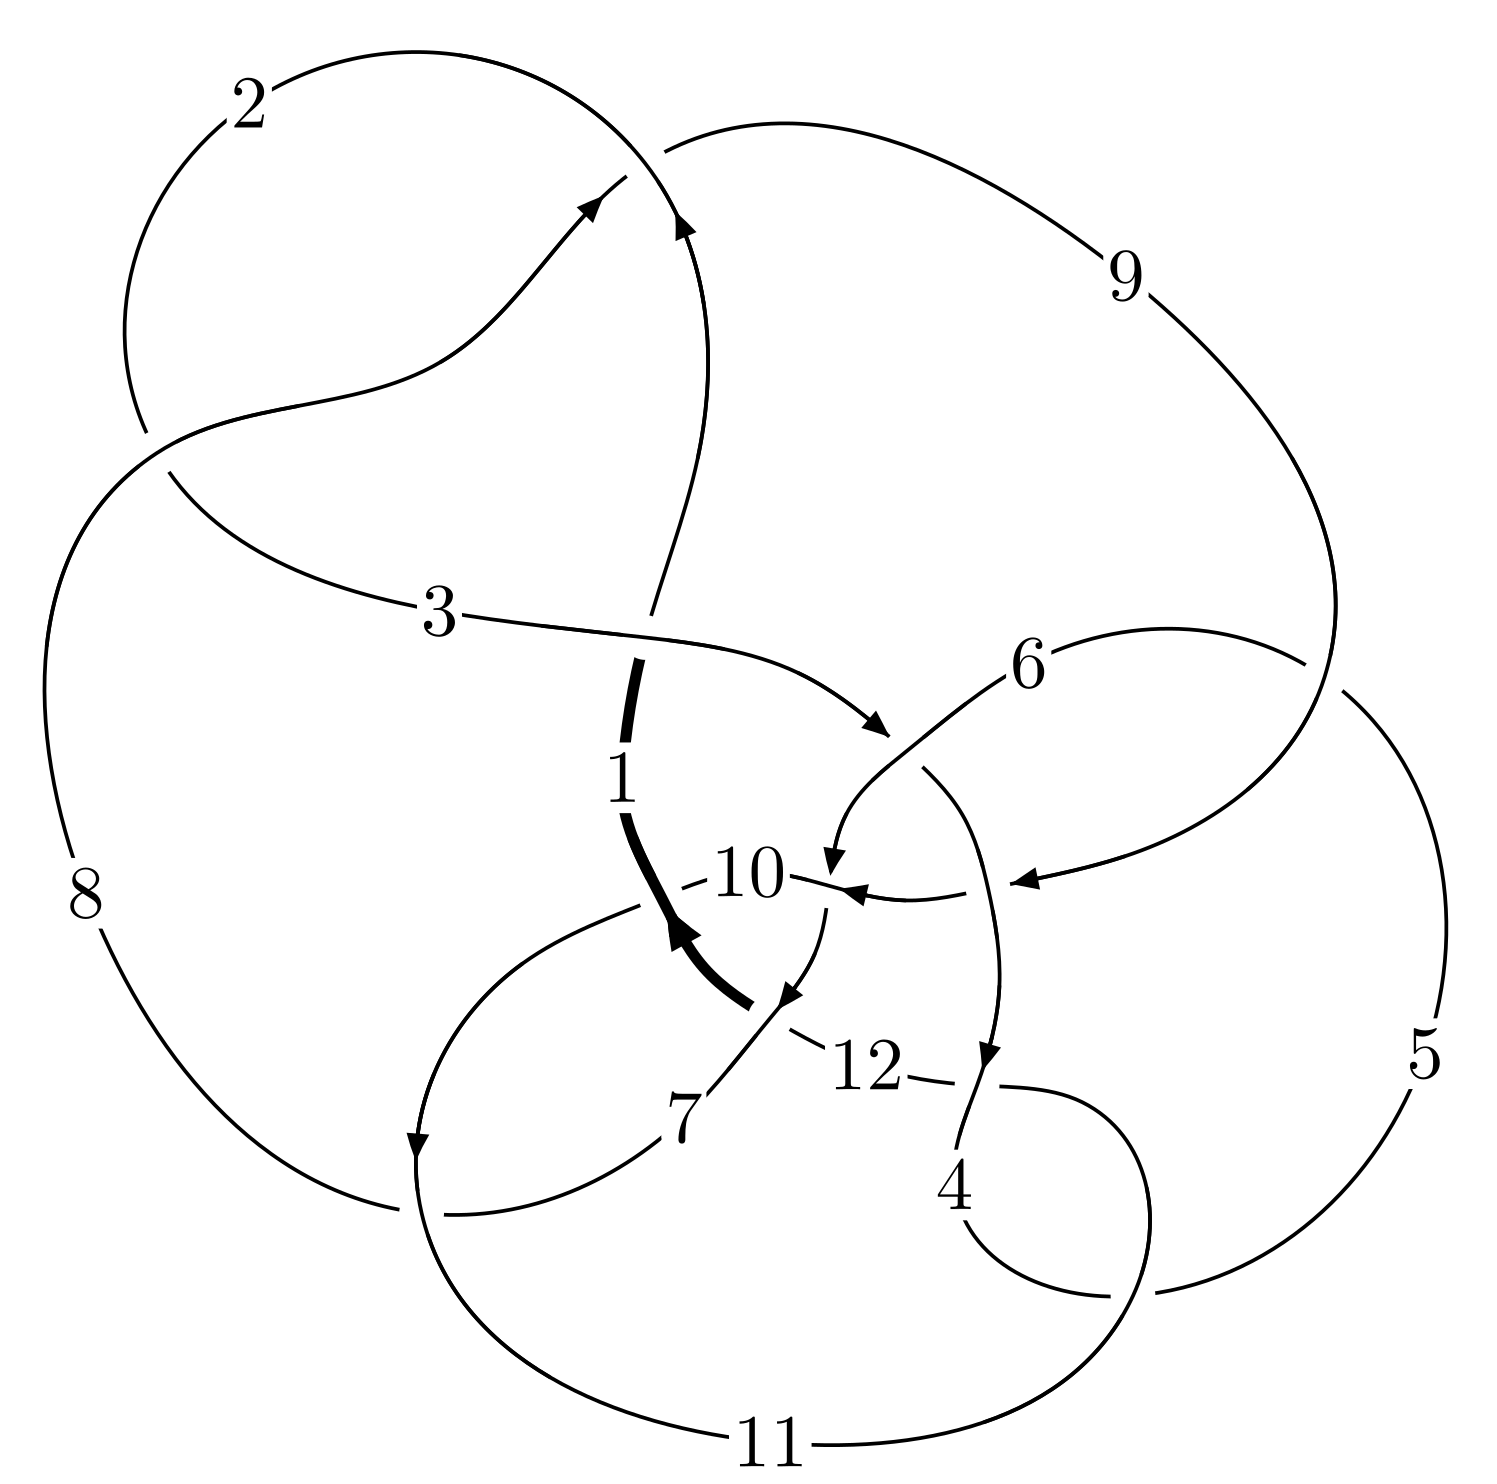
\includegraphics[width=112pt]{../../../GIT/diagram.site/Diagrams/png/2721_12n_0632.png}\\
\ \ \ A knot diagram\footnotemark}&
\allowdisplaybreaks
\textbf{Linearized knot diagam} \\
\cline{2-2}
 &
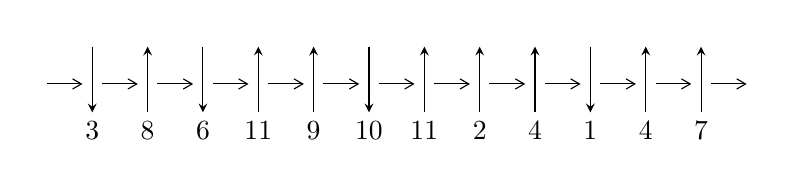
\begin{tikzpicture}[x=20pt, y=17pt]
	% nodes
	\node (C0) at (0, 0) {};
	\node (C1) at (1, 0) {};
	\node (C1U) at (1, +1) {};
	\node (C1D) at (1, -1) {3};

	\node (C2) at (2, 0) {};
	\node (C2U) at (2, +1) {};
	\node (C2D) at (2, -1) {8};

	\node (C3) at (3, 0) {};
	\node (C3U) at (3, +1) {};
	\node (C3D) at (3, -1) {6};

	\node (C4) at (4, 0) {};
	\node (C4U) at (4, +1) {};
	\node (C4D) at (4, -1) {11};

	\node (C5) at (5, 0) {};
	\node (C5U) at (5, +1) {};
	\node (C5D) at (5, -1) {9};

	\node (C6) at (6, 0) {};
	\node (C6U) at (6, +1) {};
	\node (C6D) at (6, -1) {10};

	\node (C7) at (7, 0) {};
	\node (C7U) at (7, +1) {};
	\node (C7D) at (7, -1) {11};

	\node (C8) at (8, 0) {};
	\node (C8U) at (8, +1) {};
	\node (C8D) at (8, -1) {2};

	\node (C9) at (9, 0) {};
	\node (C9U) at (9, +1) {};
	\node (C9D) at (9, -1) {4};

	\node (C10) at (10, 0) {};
	\node (C10U) at (10, +1) {};
	\node (C10D) at (10, -1) {1};

	\node (C11) at (11, 0) {};
	\node (C11U) at (11, +1) {};
	\node (C11D) at (11, -1) {4};

	\node (C12) at (12, 0) {};
	\node (C12U) at (12, +1) {};
	\node (C12D) at (12, -1) {7};
	\node (C13) at (13, 0) {};

	% arrows
	\draw[->,>={angle 60}]
	(C0) edge (C1) (C1) edge (C2) (C2) edge (C3) (C3) edge (C4) (C4) edge (C5) (C5) edge (C6) (C6) edge (C7) (C7) edge (C8) (C8) edge (C9) (C9) edge (C10) (C10) edge (C11) (C11) edge (C12) (C12) edge (C13) ;	\draw[->,>=stealth]
	(C1U) edge (C1D) (C2D) edge (C2U) (C3U) edge (C3D) (C4D) edge (C4U) (C5D) edge (C5U) (C6U) edge (C6D) (C7D) edge (C7U) (C8D) edge (C8U) (C9D) edge (C9U) (C10U) edge (C10D) (C11D) edge (C11U) (C12D) edge (C12U) ;
	\end{tikzpicture} \\
\hhline{~~} \\& 
\textbf{Solving Sequence} \\ \cline{2-2} 
 &
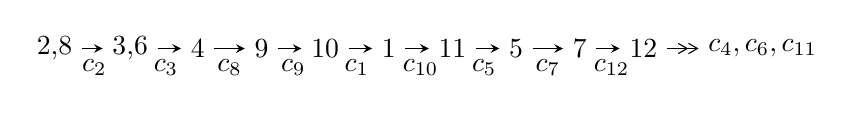
\begin{tikzpicture}[x=23pt, y=7pt]
	% node
	\node (A0) at (-1/8, 0) {2,8};
	\node (A1) at (17/16, 0) {3,6};
	\node (A2) at (17/8, 0) {4};
	\node (A3) at (25/8, 0) {9};
	\node (A4) at (33/8, 0) {10};
	\node (A5) at (41/8, 0) {1};
	\node (A6) at (49/8, 0) {11};
	\node (A7) at (57/8, 0) {5};
	\node (A8) at (65/8, 0) {7};
	\node (A9) at (73/8, 0) {12};
	\node (C1) at (1/2, -1) {$c_{2}$};
	\node (C2) at (13/8, -1) {$c_{3}$};
	\node (C3) at (21/8, -1) {$c_{8}$};
	\node (C4) at (29/8, -1) {$c_{9}$};
	\node (C5) at (37/8, -1) {$c_{1}$};
	\node (C6) at (45/8, -1) {$c_{10}$};
	\node (C7) at (53/8, -1) {$c_{5}$};
	\node (C8) at (61/8, -1) {$c_{7}$};
	\node (C9) at (69/8, -1) {$c_{12}$};
	\node (A10) at (11, 0) {$c_{4},c_{6},c_{11}$};

	% edge
	\draw[->,>=stealth]	
	(A0) edge (A1) (A1) edge (A2) (A2) edge (A3) (A3) edge (A4) (A4) edge (A5) (A5) edge (A6) (A6) edge (A7) (A7) edge (A8) (A8) edge (A9) ;
	\draw[->>,>={angle 60}]	
	(A9) edge (A10);
\end{tikzpicture} \\ 

\end{tabular} \\

\footnotetext{
The image of knot diagram is generated by the software ``\textbf{Draw programme}" developed by Andrew Bartholomew(\url{http://www.layer8.co.uk/maths/draw/index.htm\#Running-draw}), where we modified some parts for our purpose(\url{https://github.com/CATsTAILs/LinksPainter}).
}\phantom \\ \newline 
\centering \textbf{Ideals for irreducible components\footnotemark of $X_{\text{par}}$} 
 
\begin{align*}
I^u_{1}&=\langle 
2.90187\times10^{41} u^{47}-3.78001\times10^{41} u^{46}+\cdots+1.28153\times10^{42} b+4.17139\times10^{42},\\
\phantom{I^u_{1}}&\phantom{= \langle  }3.62446\times10^{41} u^{47}-9.89184\times10^{41} u^{46}+\cdots+5.12610\times10^{42} a+3.33997\times10^{42},\;u^{48}-3 u^{47}+\cdots-72 u+16\rangle \\
I^u_{2}&=\langle 
-2.03008\times10^{16} a u^{32}+2.90523\times10^{16} u^{32}+\cdots-2.34244\times10^{17} a+2.23321\times10^{17},\\
\phantom{I^u_{2}}&\phantom{= \langle  }-1.75837\times10^{15} a u^{32}-3.99178\times10^{16} u^{32}+\cdots-3.28264\times10^{17} a+3.99087\times10^{17},\\
\phantom{I^u_{2}}&\phantom{= \langle  }u^{33}+u^{32}+\cdots-7 u+11\rangle \\
I^u_{3}&=\langle 
825341 u^{37}+1493 u^{36}+\cdots+121486 b-2500187,\\
\phantom{I^u_{3}}&\phantom{= \langle  }2974391 u^{37}-2651575 u^{36}+\cdots+607430 a-22087770,\;u^{38}+11 u^{36}+\cdots+12 u^2+5\rangle \\
\\
I^v_{1}&=\langle 
a,\;v^2+b+2 v,\;v^3+3 v^2+2 v+1\rangle \\
\end{align*}
\raggedright * 4 irreducible components of $\dim_{\mathbb{C}}=0$, with total 155 representations.\\
\footnotetext{All coefficients of polynomials are rational numbers. But the coefficients are sometimes approximated in decimal forms when there is not enough margin.}
\newpage
\renewcommand{\arraystretch}{1}
\centering \section*{I. $I^u_{1}= \langle 2.90\times10^{41} u^{47}-3.78\times10^{41} u^{46}+\cdots+1.28\times10^{42} b+4.17\times10^{42},\;3.62\times10^{41} u^{47}-9.89\times10^{41} u^{46}+\cdots+5.13\times10^{42} a+3.34\times10^{42},\;u^{48}-3 u^{47}+\cdots-72 u+16 \rangle$}
\flushleft \textbf{(i) Arc colorings}\\
\begin{tabular}{m{7pt} m{180pt} m{7pt} m{180pt} }
\flushright $a_{2}=$&$\begin{pmatrix}1\\0\end{pmatrix}$ \\
\flushright $a_{8}=$&$\begin{pmatrix}0\\u\end{pmatrix}$ \\
\flushright $a_{3}=$&$\begin{pmatrix}1\\- u^2\end{pmatrix}$ \\
\flushright $a_{6}=$&$\begin{pmatrix}-0.0707059 u^{47}+0.192970 u^{46}+\cdots+2.02201 u-0.651561\\-0.226439 u^{47}+0.294962 u^{46}+\cdots+10.9693 u-3.25501\end{pmatrix}$ \\
\flushright $a_{4}=$&$\begin{pmatrix}-0.510598 u^{47}+1.08091 u^{46}+\cdots-13.9117 u+2.18945\\-0.454714 u^{47}+0.887793 u^{46}+\cdots+1.07657 u-2.81659\end{pmatrix}$ \\
\flushright $a_{9}=$&$\begin{pmatrix}u\\u\end{pmatrix}$ \\
\flushright $a_{10}=$&$\begin{pmatrix}-0.294663 u^{47}+0.316302 u^{46}+\cdots+9.54700 u-3.10520\\0.0653557 u^{47}-0.679568 u^{46}+\cdots+37.0059 u-9.89112\end{pmatrix}$ \\
\flushright $a_{1}=$&$\begin{pmatrix}u^2+1\\- u^4\end{pmatrix}$ \\
\flushright $a_{11}=$&$\begin{pmatrix}-0.155733 u^{47}+0.101992 u^{46}+\cdots+8.94734 u-2.60345\\-0.0000489054 u^{47}-0.477796 u^{46}+\cdots+34.7725 u-9.09833\end{pmatrix}$ \\
\flushright $a_{5}=$&$\begin{pmatrix}0.155684 u^{47}-0.579788 u^{46}+\cdots+25.8252 u-6.49488\\-0.0000489054 u^{47}-0.477796 u^{46}+\cdots+34.7725 u-9.09833\end{pmatrix}$ \\
\flushright $a_{7}=$&$\begin{pmatrix}0.700023 u^{47}-1.69491 u^{46}+\cdots+31.7696 u-6.01626\\0.500164 u^{47}-1.27854 u^{46}+\cdots+19.1631 u-1.82344\end{pmatrix}$ \\
\flushright $a_{12}=$&$\begin{pmatrix}0.569045 u^{47}-0.934017 u^{46}+\cdots+6.75968 u+0.801632\\-0.0171747 u^{47}+0.560556 u^{46}+\cdots-33.6917 u+10.3628\end{pmatrix}$\\&\end{tabular}
\flushleft \textbf{(ii) Obstruction class $= -1$}\\~\\
\flushleft \textbf{(iii) Cusp Shapes $= -2.71002 u^{47}+7.94048 u^{46}+\cdots-215.263 u+55.9379$}\\~\\
\newpage\renewcommand{\arraystretch}{1}
\flushleft \textbf{(iv) u-Polynomials at the component}\newline \\
\begin{tabular}{m{50pt}|m{274pt}}
Crossings & \hspace{64pt}u-Polynomials at each crossing \\
\hline $$\begin{aligned}c_{1}\end{aligned}$$&$\begin{aligned}
&u^{48}+23 u^{47}+\cdots+832 u+256
\end{aligned}$\\
\hline $$\begin{aligned}c_{2},c_{8}\end{aligned}$$&$\begin{aligned}
&u^{48}+3 u^{47}+\cdots+72 u+16
\end{aligned}$\\
\hline $$\begin{aligned}c_{3},c_{10}\end{aligned}$$&$\begin{aligned}
&u^{48}- u^{47}+\cdots-3 u+1
\end{aligned}$\\
\hline $$\begin{aligned}c_{4},c_{11}\end{aligned}$$&$\begin{aligned}
&u^{48}-5 u^{47}+\cdots-1329 u+160
\end{aligned}$\\
\hline $$\begin{aligned}c_{5},c_{7}\end{aligned}$$&$\begin{aligned}
&u^{48}-22 u^{46}+\cdots+700 u+200
\end{aligned}$\\
\hline $$\begin{aligned}c_{6}\end{aligned}$$&$\begin{aligned}
&u^{48}+6 u^{47}+\cdots-2475 u+918
\end{aligned}$\\
\hline $$\begin{aligned}c_{9},c_{12}\end{aligned}$$&$\begin{aligned}
&u^{48}-16 u^{46}+\cdots-154 u+17
\end{aligned}$\\
\hline
\end{tabular}\\~\\
\newpage\renewcommand{\arraystretch}{1}
\flushleft \textbf{(v) Riley Polynomials at the component}\newline \\
\begin{tabular}{m{50pt}|m{274pt}}
Crossings & \hspace{64pt}Riley Polynomials at each crossing \\
\hline $$\begin{aligned}c_{1}\end{aligned}$$&$\begin{aligned}
&y^{48}+11 y^{47}+\cdots+675840 y+65536
\end{aligned}$\\
\hline $$\begin{aligned}c_{2},c_{8}\end{aligned}$$&$\begin{aligned}
&y^{48}+23 y^{47}+\cdots+832 y+256
\end{aligned}$\\
\hline $$\begin{aligned}c_{3},c_{10}\end{aligned}$$&$\begin{aligned}
&y^{48}- y^{47}+\cdots+27 y+1
\end{aligned}$\\
\hline $$\begin{aligned}c_{4},c_{11}\end{aligned}$$&$\begin{aligned}
&y^{48}-37 y^{47}+\cdots-197281 y+25600
\end{aligned}$\\
\hline $$\begin{aligned}c_{5},c_{7}\end{aligned}$$&$\begin{aligned}
&y^{48}-44 y^{47}+\cdots+2167600 y+40000
\end{aligned}$\\
\hline $$\begin{aligned}c_{6}\end{aligned}$$&$\begin{aligned}
&y^{48}+2 y^{47}+\cdots-1509921 y+842724
\end{aligned}$\\
\hline $$\begin{aligned}c_{9},c_{12}\end{aligned}$$&$\begin{aligned}
&y^{48}-32 y^{47}+\cdots-15386 y+289
\end{aligned}$\\
\hline
\end{tabular}\\~\\
\newpage\flushleft \textbf{(vi) Complex Volumes and Cusp Shapes}
$$\begin{array}{c|c|c}  
\text{Solutions to }I^u_{1}& \I (\text{vol} + \sqrt{-1}CS) & \text{Cusp shape}\\
 \hline 
\begin{aligned}
u &= -0.072234 + 1.009590 I \\
a &= -1.22324 + 0.93575 I \\
b &= -0.322776 + 0.234343 I\end{aligned}
 & -3.79904 + 3.93017 I & -1.59134 - 4.51288 I \\ \hline\begin{aligned}
u &= -0.072234 - 1.009590 I \\
a &= -1.22324 - 0.93575 I \\
b &= -0.322776 - 0.234343 I\end{aligned}
 & -3.79904 - 3.93017 I & -1.59134 + 4.51288 I \\ \hline\begin{aligned}
u &= -0.750282 + 0.624427 I \\
a &= \phantom{-}0.877939 - 0.849112 I \\
b &= \phantom{-}1.83705 + 0.04183 I\end{aligned}
 & \phantom{-}1.29000 + 4.48373 I & \phantom{-}7.58276 - 2.87666 I \\ \hline\begin{aligned}
u &= -0.750282 - 0.624427 I \\
a &= \phantom{-}0.877939 + 0.849112 I \\
b &= \phantom{-}1.83705 - 0.04183 I\end{aligned}
 & \phantom{-}1.29000 - 4.48373 I & \phantom{-}7.58276 + 2.87666 I \\ \hline\begin{aligned}
u &= \phantom{-}0.613049 + 0.734079 I \\
a &= \phantom{-}0.34365 + 2.29466 I \\
b &= \phantom{-}1.075750 + 0.555261 I\end{aligned}
 & \phantom{-}6.97125 + 0.95587 I & \phantom{-}6.61091 - 4.11301 I \\ \hline\begin{aligned}
u &= \phantom{-}0.613049 - 0.734079 I \\
a &= \phantom{-}0.34365 - 2.29466 I \\
b &= \phantom{-}1.075750 - 0.555261 I\end{aligned}
 & \phantom{-}6.97125 - 0.95587 I & \phantom{-}6.61091 + 4.11301 I \\ \hline\begin{aligned}
u &= \phantom{-}0.713580 + 0.617959 I \\
a &= \phantom{-}0.903291 + 0.979506 I \\
b &= \phantom{-}1.020980 + 0.018093 I\end{aligned}
 & \phantom{-}1.77056 - 2.17781 I & \phantom{-}4.82468 + 3.78261 I \\ \hline\begin{aligned}
u &= \phantom{-}0.713580 - 0.617959 I \\
a &= \phantom{-}0.903291 - 0.979506 I \\
b &= \phantom{-}1.020980 - 0.018093 I\end{aligned}
 & \phantom{-}1.77056 + 2.17781 I & \phantom{-}4.82468 - 3.78261 I \\ \hline\begin{aligned}
u &= -0.106932 + 1.050970 I \\
a &= \phantom{-}0.513607 + 0.490726 I \\
b &= -0.13366 + 1.43900 I\end{aligned}
 & \phantom{-}2.12023 + 1.00595 I & \phantom{-}5.23912 - 2.50505 I \\ \hline\begin{aligned}
u &= -0.106932 - 1.050970 I \\
a &= \phantom{-}0.513607 - 0.490726 I \\
b &= -0.13366 - 1.43900 I\end{aligned}
 & \phantom{-}2.12023 - 1.00595 I & \phantom{-}5.23912 + 2.50505 I\\
 \hline 
 \end{array}$$\newpage$$\begin{array}{c|c|c}  
\text{Solutions to }I^u_{1}& \I (\text{vol} + \sqrt{-1}CS) & \text{Cusp shape}\\
 \hline 
\begin{aligned}
u &= \phantom{-}0.998142 + 0.481752 I \\
a &= -0.639140 - 1.033170 I \\
b &= -1.61536 + 0.35291 I\end{aligned}
 & \phantom{-}7.2965 - 12.6756 I & \phantom{-}6.45387 + 5.95608 I \\ \hline\begin{aligned}
u &= \phantom{-}0.998142 - 0.481752 I \\
a &= -0.639140 + 1.033170 I \\
b &= -1.61536 - 0.35291 I\end{aligned}
 & \phantom{-}7.2965 + 12.6756 I & \phantom{-}6.45387 - 5.95608 I \\ \hline\begin{aligned}
u &= -0.745488 + 0.467501 I \\
a &= -0.40070 + 1.92827 I \\
b &= -1.63796 - 0.07983 I\end{aligned}
 & \phantom{-}7.04207 + 2.69361 I & \phantom{-}12.38588 - 5.07908 I \\ \hline\begin{aligned}
u &= -0.745488 - 0.467501 I \\
a &= -0.40070 - 1.92827 I \\
b &= -1.63796 + 0.07983 I\end{aligned}
 & \phantom{-}7.04207 - 2.69361 I & \phantom{-}12.38588 + 5.07908 I \\ \hline\begin{aligned}
u &= \phantom{-}0.364690 + 1.059660 I \\
a &= -0.117822 - 0.681542 I \\
b &= \phantom{-}0.234019 - 0.185992 I\end{aligned}
 & -3.73555 + 0.62051 I & \phantom{-0.000000 } 0 \\ \hline\begin{aligned}
u &= \phantom{-}0.364690 - 1.059660 I \\
a &= -0.117822 + 0.681542 I \\
b &= \phantom{-}0.234019 + 0.185992 I\end{aligned}
 & -3.73555 - 0.62051 I & \phantom{-0.000000 } 0 \\ \hline\begin{aligned}
u &= \phantom{-}0.451904 + 1.026910 I \\
a &= -1.33410 - 1.30797 I \\
b &= -1.32090 - 0.59244 I\end{aligned}
 & -3.32273 + 6.10549 I & \phantom{-0.000000 } 0. - 6.61286 I \\ \hline\begin{aligned}
u &= \phantom{-}0.451904 - 1.026910 I \\
a &= -1.33410 + 1.30797 I \\
b &= -1.32090 + 0.59244 I\end{aligned}
 & -3.32273 - 6.10549 I & \phantom{-0.000000 -}0. + 6.61286 I \\ \hline\begin{aligned}
u &= \phantom{-}0.640017 + 0.942419 I \\
a &= -0.820679 - 0.511384 I \\
b &= -1.96429 - 0.04776 I\end{aligned}
 & \phantom{-}6.31587 + 4.00200 I & \phantom{-}6.45296 - 3.11892 I \\ \hline\begin{aligned}
u &= \phantom{-}0.640017 - 0.942419 I \\
a &= -0.820679 + 0.511384 I \\
b &= -1.96429 + 0.04776 I\end{aligned}
 & \phantom{-}6.31587 - 4.00200 I & \phantom{-}6.45296 + 3.11892 I\\
 \hline 
 \end{array}$$\newpage$$\begin{array}{c|c|c}  
\text{Solutions to }I^u_{1}& \I (\text{vol} + \sqrt{-1}CS) & \text{Cusp shape}\\
 \hline 
\begin{aligned}
u &= \phantom{-}0.298498 + 0.789976 I \\
a &= \phantom{-}0.379370 + 0.964150 I \\
b &= \phantom{-}1.56784 + 1.18772 I\end{aligned}
 & -2.12114 - 2.96147 I & -3.25494 + 1.48217 I \\ \hline\begin{aligned}
u &= \phantom{-}0.298498 - 0.789976 I \\
a &= \phantom{-}0.379370 - 0.964150 I \\
b &= \phantom{-}1.56784 - 1.18772 I\end{aligned}
 & -2.12114 + 2.96147 I & -3.25494 - 1.48217 I \\ \hline\begin{aligned}
u &= -0.463720 + 1.068040 I \\
a &= \phantom{-}0.874078 - 0.695825 I \\
b &= \phantom{-}0.872961 - 0.051243 I\end{aligned}
 & -1.10916 - 3.41423 I & \phantom{-0.000000 } 0 \\ \hline\begin{aligned}
u &= -0.463720 - 1.068040 I \\
a &= \phantom{-}0.874078 + 0.695825 I \\
b &= \phantom{-}0.872961 + 0.051243 I\end{aligned}
 & -1.10916 + 3.41423 I & \phantom{-0.000000 } 0 \\ \hline\begin{aligned}
u &= \phantom{-}0.637391 + 0.990955 I \\
a &= -0.45612 - 1.38999 I \\
b &= -1.52449 - 1.28957 I\end{aligned}
 & \phantom{-}0.68173 + 7.36598 I & \phantom{-0.000000 } 0. - 8.55059 I \\ \hline\begin{aligned}
u &= \phantom{-}0.637391 - 0.990955 I \\
a &= -0.45612 + 1.38999 I \\
b &= -1.52449 + 1.28957 I\end{aligned}
 & \phantom{-}0.68173 - 7.36598 I & \phantom{-0.000000 -}0. + 8.55059 I \\ \hline\begin{aligned}
u &= -0.663005 + 1.024610 I \\
a &= -0.75487 + 1.93333 I \\
b &= -1.74471 + 1.01235 I\end{aligned}
 & \phantom{-}0.08239 - 9.87726 I & \phantom{-0.000000 } 0 \\ \hline\begin{aligned}
u &= -0.663005 - 1.024610 I \\
a &= -0.75487 - 1.93333 I \\
b &= -1.74471 - 1.01235 I\end{aligned}
 & \phantom{-}0.08239 + 9.87726 I & \phantom{-0.000000 } 0 \\ \hline\begin{aligned}
u &= -1.056260 + 0.636872 I \\
a &= -0.032565 - 1.010660 I \\
b &= \phantom{-}0.789001 - 0.401945 I\end{aligned}
 & \phantom{-}8.12208 - 6.43854 I & \phantom{-0.000000 } 0 \\ \hline\begin{aligned}
u &= -1.056260 - 0.636872 I \\
a &= -0.032565 + 1.010660 I \\
b &= \phantom{-}0.789001 + 0.401945 I\end{aligned}
 & \phantom{-}8.12208 + 6.43854 I & \phantom{-0.000000 } 0\\
 \hline 
 \end{array}$$\newpage$$\begin{array}{c|c|c}  
\text{Solutions to }I^u_{1}& \I (\text{vol} + \sqrt{-1}CS) & \text{Cusp shape}\\
 \hline 
\begin{aligned}
u &= -0.606495 + 1.075940 I \\
a &= \phantom{-}1.00711 - 1.81965 I \\
b &= \phantom{-}2.69461 - 1.04799 I\end{aligned}
 & \phantom{-}5.24428 - 7.84216 I & \phantom{-0.000000 } 0 \\ \hline\begin{aligned}
u &= -0.606495 - 1.075940 I \\
a &= \phantom{-}1.00711 + 1.81965 I \\
b &= \phantom{-}2.69461 + 1.04799 I\end{aligned}
 & \phantom{-}5.24428 + 7.84216 I & \phantom{-0.000000 } 0 \\ \hline\begin{aligned}
u &= \phantom{-}0.648933 + 0.372189 I \\
a &= -1.15793 + 1.69242 I \\
b &= \phantom{-}0.844553 + 0.510508 I\end{aligned}
 & \phantom{-}6.95234 + 0.39618 I & \phantom{-}12.53507 - 4.08831 I \\ \hline\begin{aligned}
u &= \phantom{-}0.648933 - 0.372189 I \\
a &= -1.15793 - 1.69242 I \\
b &= \phantom{-}0.844553 - 0.510508 I\end{aligned}
 & \phantom{-}6.95234 - 0.39618 I & \phantom{-}12.53507 + 4.08831 I \\ \hline\begin{aligned}
u &= \phantom{-}0.563635 + 1.174740 I \\
a &= -0.951010 - 0.642156 I \\
b &= -1.75643 + 0.28005 I\end{aligned}
 & \phantom{-}4.46125 + 4.40033 I & \phantom{-0.000000 } 0 \\ \hline\begin{aligned}
u &= \phantom{-}0.563635 - 1.174740 I \\
a &= -0.951010 + 0.642156 I \\
b &= -1.75643 - 0.28005 I\end{aligned}
 & \phantom{-}4.46125 - 4.40033 I & \phantom{-0.000000 } 0 \\ \hline\begin{aligned}
u &= \phantom{-}0.705215 + 1.162730 I \\
a &= \phantom{-}0.82971 + 1.66340 I \\
b &= \phantom{-}2.21819 + 1.08373 I\end{aligned}
 & \phantom{-}5.1858 + 18.8530 I & \phantom{-0.000000 } 0 \\ \hline\begin{aligned}
u &= \phantom{-}0.705215 - 1.162730 I \\
a &= \phantom{-}0.82971 - 1.66340 I \\
b &= \phantom{-}2.21819 - 1.08373 I\end{aligned}
 & \phantom{-}5.1858 - 18.8530 I & \phantom{-0.000000 } 0 \\ \hline\begin{aligned}
u &= \phantom{-}0.613806 + 0.078399 I \\
a &= \phantom{-}0.529727 - 0.797181 I \\
b &= \phantom{-}0.548360 - 0.505925 I\end{aligned}
 & -0.74503 + 2.83022 I & \phantom{-}7.38869 - 2.36983 I \\ \hline\begin{aligned}
u &= \phantom{-}0.613806 - 0.078399 I \\
a &= \phantom{-}0.529727 + 0.797181 I \\
b &= \phantom{-}0.548360 + 0.505925 I\end{aligned}
 & -0.74503 - 2.83022 I & \phantom{-}7.38869 + 2.36983 I\\
 \hline 
 \end{array}$$\newpage$$\begin{array}{c|c|c}  
\text{Solutions to }I^u_{1}& \I (\text{vol} + \sqrt{-1}CS) & \text{Cusp shape}\\
 \hline 
\begin{aligned}
u &= -0.500797 + 0.350954 I \\
a &= \phantom{-}0.320846 + 0.457891 I \\
b &= -0.431234 + 0.483909 I\end{aligned}
 & \phantom{-}0.956146 - 0.504632 I & \phantom{-}9.17940 + 3.83818 I \\ \hline\begin{aligned}
u &= -0.500797 - 0.350954 I \\
a &= \phantom{-}0.320846 - 0.457891 I \\
b &= -0.431234 - 0.483909 I\end{aligned}
 & \phantom{-}0.956146 + 0.504632 I & \phantom{-}9.17940 - 3.83818 I \\ \hline\begin{aligned}
u &= \phantom{-}0.001378 + 1.393570 I \\
a &= \phantom{-}0.499786 + 0.079532 I \\
b &= \phantom{-}0.035284 - 0.688867 I\end{aligned}
 & \phantom{-}0.18184 - 9.53195 I & \phantom{-0.000000 } 0 \\ \hline\begin{aligned}
u &= \phantom{-}0.001378 - 1.393570 I \\
a &= \phantom{-}0.499786 - 0.079532 I \\
b &= \phantom{-}0.035284 + 0.688867 I\end{aligned}
 & \phantom{-}0.18184 + 9.53195 I & \phantom{-0.000000 } 0 \\ \hline\begin{aligned}
u &= -0.870155 + 1.110250 I \\
a &= -0.623696 + 0.359289 I \\
b &= -1.309200 + 0.026773 I\end{aligned}
 & \phantom{-}6.69908 - 0.43812 I & \phantom{-0.000000 } 0 \\ \hline\begin{aligned}
u &= -0.870155 - 1.110250 I \\
a &= -0.623696 - 0.359289 I \\
b &= -1.309200 - 0.026773 I\end{aligned}
 & \phantom{-}6.69908 + 0.43812 I & \phantom{-0.000000 } 0 \\ \hline\begin{aligned}
u &= \phantom{-}0.08513 + 1.42831 I \\
a &= \phantom{-}0.182771 - 0.302780 I \\
b &= \phantom{-}0.522416 - 0.131488 I\end{aligned}
 & -4.72528 - 0.59037 I & \phantom{-0.000000 } 0 \\ \hline\begin{aligned}
u &= \phantom{-}0.08513 - 1.42831 I \\
a &= \phantom{-}0.182771 + 0.302780 I \\
b &= \phantom{-}0.522416 + 0.131488 I\end{aligned}
 & -4.72528 + 0.59037 I & \phantom{-0.000000 } 0\\
 \hline 
 \end{array}$$\newpage\newpage\renewcommand{\arraystretch}{1}
\centering \section*{II. $I^u_{2}= \langle -2.03\times10^{16} a u^{32}+2.91\times10^{16} u^{32}+\cdots-2.34\times10^{17} a+2.23\times10^{17},\;-1.76\times10^{15} a u^{32}-3.99\times10^{16} u^{32}+\cdots-3.28\times10^{17} a+3.99\times10^{17},\;u^{33}+u^{32}+\cdots-7 u+11 \rangle$}
\flushleft \textbf{(i) Arc colorings}\\
\begin{tabular}{m{7pt} m{180pt} m{7pt} m{180pt} }
\flushright $a_{2}=$&$\begin{pmatrix}1\\0\end{pmatrix}$ \\
\flushright $a_{8}=$&$\begin{pmatrix}0\\u\end{pmatrix}$ \\
\flushright $a_{3}=$&$\begin{pmatrix}1\\- u^2\end{pmatrix}$ \\
\flushright $a_{6}=$&$\begin{pmatrix}a\\0.391169 a u^{32}-0.559799 u^{32}+\cdots+4.51357 a-4.30309\end{pmatrix}$ \\
\flushright $a_{4}=$&$\begin{pmatrix}0.364219 a u^{32}+0.464300 u^{32}+\cdots+2.24836 a-22.1496\\0.234314 a u^{32}+0.527041 u^{32}+\cdots-0.198158 a-16.6316\end{pmatrix}$ \\
\flushright $a_{9}=$&$\begin{pmatrix}u\\u\end{pmatrix}$ \\
\flushright $a_{10}=$&$\begin{pmatrix}-0.264790 a u^{32}+0.618972 u^{32}+\cdots-2.62489 a-3.56836\\-0.780172 a u^{32}-0.142686 u^{32}+\cdots-8.71610 a-3.79069\end{pmatrix}$ \\
\flushright $a_{1}=$&$\begin{pmatrix}u^2+1\\- u^4\end{pmatrix}$ \\
\flushright $a_{11}=$&$\begin{pmatrix}-0.391169 a u^{32}-0.114073 u^{32}+\cdots-3.51357 a-4.91800\\-0.908717 a u^{32}-0.584667 u^{32}+\cdots-9.91583 a+0.416754\end{pmatrix}$ \\
\flushright $a_{5}=$&$\begin{pmatrix}0.517548 a u^{32}+0.341193 u^{32}+\cdots+6.40225 a-2.21651\\0.908717 a u^{32}-0.218606 u^{32}+\cdots+9.91583 a-6.51960\end{pmatrix}$ \\
\flushright $a_{7}=$&$\begin{pmatrix}0.908250 a u^{32}+2.38664 u^{32}+\cdots+5.60633 a+2.84026\\0.989039 a u^{32}+2.76675 u^{32}+\cdots+0.911866 a-0.529176\end{pmatrix}$ \\
\flushright $a_{12}=$&$\begin{pmatrix}-0.620353 a u^{32}+0.737707 u^{32}+\cdots+10.6936 a+9.69735\\0.315026 a u^{32}+1.68970 u^{32}+\cdots+17.0382 a+7.83841\end{pmatrix}$\\&\end{tabular}
\flushleft \textbf{(ii) Obstruction class $= -1$}\\~\\
\flushleft \textbf{(iii) Cusp Shapes $= \frac{903243108544774}{625274099350525} u^{32}+\frac{1805117122242941}{625274099350525} u^{31}+\cdots+\frac{4314310509574099}{125054819870105} u-\frac{11096996532907333}{625274099350525}$}\\~\\
\newpage\renewcommand{\arraystretch}{1}
\flushleft \textbf{(iv) u-Polynomials at the component}\newline \\
\begin{tabular}{m{50pt}|m{274pt}}
Crossings & \hspace{64pt}u-Polynomials at each crossing \\
\hline $$\begin{aligned}c_{1}\end{aligned}$$&$\begin{aligned}
&(u^{33}+13 u^{32}+\cdots-941 u-121)^{2}
\end{aligned}$\\
\hline $$\begin{aligned}c_{2},c_{8}\end{aligned}$$&$\begin{aligned}
&(u^{33}- u^{32}+\cdots-7 u-11)^{2}
\end{aligned}$\\
\hline $$\begin{aligned}c_{3},c_{10}\end{aligned}$$&$\begin{aligned}
&u^{66}-7 u^{65}+\cdots+47 u+29
\end{aligned}$\\
\hline $$\begin{aligned}c_{4},c_{11}\end{aligned}$$&$\begin{aligned}
&(u^{33}+2 u^{32}+\cdots-8 u-1)^{2}
\end{aligned}$\\
\hline $$\begin{aligned}c_{5},c_{7}\end{aligned}$$&$\begin{aligned}
&u^{66}+12 u^{64}+\cdots-1048425 u-638825
\end{aligned}$\\
\hline $$\begin{aligned}c_{6}\end{aligned}$$&$\begin{aligned}
&(u^{33}- u^{32}+\cdots-4 u-1)^{2}
\end{aligned}$\\
\hline $$\begin{aligned}c_{9},c_{12}\end{aligned}$$&$\begin{aligned}
&u^{66}-2 u^{65}+\cdots-52649 u-9793
\end{aligned}$\\
\hline
\end{tabular}\\~\\
\newpage\renewcommand{\arraystretch}{1}
\flushleft \textbf{(v) Riley Polynomials at the component}\newline \\
\begin{tabular}{m{50pt}|m{274pt}}
Crossings & \hspace{64pt}Riley Polynomials at each crossing \\
\hline $$\begin{aligned}c_{1}\end{aligned}$$&$\begin{aligned}
&(y^{33}+17 y^{32}+\cdots+5327 y-14641)^{2}
\end{aligned}$\\
\hline $$\begin{aligned}c_{2},c_{8}\end{aligned}$$&$\begin{aligned}
&(y^{33}+13 y^{32}+\cdots-941 y-121)^{2}
\end{aligned}$\\
\hline $$\begin{aligned}c_{3},c_{10}\end{aligned}$$&$\begin{aligned}
&y^{66}-31 y^{65}+\cdots-76101 y+841
\end{aligned}$\\
\hline $$\begin{aligned}c_{4},c_{11}\end{aligned}$$&$\begin{aligned}
&(y^{33}-28 y^{32}+\cdots+16 y-1)^{2}
\end{aligned}$\\
\hline $$\begin{aligned}c_{5},c_{7}\end{aligned}$$&$\begin{aligned}
&y^{66}+24 y^{65}+\cdots-2888276776775 y+408097380625
\end{aligned}$\\
\hline $$\begin{aligned}c_{6}\end{aligned}$$&$\begin{aligned}
&(y^{33}+11 y^{32}+\cdots-36 y-1)^{2}
\end{aligned}$\\
\hline $$\begin{aligned}c_{9},c_{12}\end{aligned}$$&$\begin{aligned}
&y^{66}+14 y^{65}+\cdots-2701564289 y+95902849
\end{aligned}$\\
\hline
\end{tabular}\\~\\
\newpage\flushleft \textbf{(vi) Complex Volumes and Cusp Shapes}
$$\begin{array}{c|c|c}  
\text{Solutions to }I^u_{2}& \I (\text{vol} + \sqrt{-1}CS) & \text{Cusp shape}\\
 \hline 
\begin{aligned}
u &= -1.00045\phantom{ +0.000000I} \\
a &= -0.729229\phantom{ +0.000000I} \\
b &= \phantom{-}0.0710552\phantom{ +0.000000I}\end{aligned}
 & \phantom{-}4.51725\phantom{ +0.000000I} & -4.11620\phantom{ +0.000000I} \\ \hline\begin{aligned}
u &= -1.00045\phantom{ +0.000000I} \\
a &= \phantom{-}0.192294\phantom{ +0.000000I} \\
b &= -1.64543\phantom{ +0.000000I}\end{aligned}
 & \phantom{-}4.51725\phantom{ +0.000000I} & -4.11620\phantom{ +0.000000I} \\ \hline\begin{aligned}
u &= -0.597418 + 0.770414 I \\
a &= -1.47977 - 0.11392 I \\
b &= \phantom{-}0.64936 - 1.68170 I\end{aligned}
 & \phantom{-}2.56250 + 2.10521 I & \phantom{-}4.05719 - 1.95522 I \\ \hline\begin{aligned}
u &= -0.597418 + 0.770414 I \\
a &= -1.65555 + 0.70942 I \\
b &= -2.06179 - 0.12173 I\end{aligned}
 & \phantom{-}2.56250 + 2.10521 I & \phantom{-}4.05719 - 1.95522 I \\ \hline\begin{aligned}
u &= -0.597418 - 0.770414 I \\
a &= -1.47977 + 0.11392 I \\
b &= \phantom{-}0.64936 + 1.68170 I\end{aligned}
 & \phantom{-}2.56250 - 2.10521 I & \phantom{-}4.05719 + 1.95522 I \\ \hline\begin{aligned}
u &= -0.597418 - 0.770414 I \\
a &= -1.65555 - 0.70942 I \\
b &= -2.06179 + 0.12173 I\end{aligned}
 & \phantom{-}2.56250 - 2.10521 I & \phantom{-}4.05719 + 1.95522 I \\ \hline\begin{aligned}
u &= -0.342707 + 0.887603 I \\
a &= -0.117440 - 0.661580 I \\
b &= -0.933048 + 0.344357 I\end{aligned}
 & \phantom{-}0.46246 + 2.22160 I & -0.67965 + 7.70078 I \\ \hline\begin{aligned}
u &= -0.342707 + 0.887603 I \\
a &= \phantom{-}1.15472 + 3.54214 I \\
b &= -1.18973 + 3.08181 I\end{aligned}
 & \phantom{-}0.46246 + 2.22160 I & -0.67965 + 7.70078 I \\ \hline\begin{aligned}
u &= -0.342707 - 0.887603 I \\
a &= -0.117440 + 0.661580 I \\
b &= -0.933048 - 0.344357 I\end{aligned}
 & \phantom{-}0.46246 - 2.22160 I & -0.67965 - 7.70078 I \\ \hline\begin{aligned}
u &= -0.342707 - 0.887603 I \\
a &= \phantom{-}1.15472 - 3.54214 I \\
b &= -1.18973 - 3.08181 I\end{aligned}
 & \phantom{-}0.46246 - 2.22160 I & -0.67965 - 7.70078 I\\
 \hline 
 \end{array}$$\newpage$$\begin{array}{c|c|c}  
\text{Solutions to }I^u_{2}& \I (\text{vol} + \sqrt{-1}CS) & \text{Cusp shape}\\
 \hline 
\begin{aligned}
u &= \phantom{-}0.465782 + 0.820583 I \\
a &= -0.460215 - 0.465452 I \\
b &= \phantom{-}0.728090 + 0.267934 I\end{aligned}
 & -3.34705 + 1.85137 I & \phantom{-}0.37014 - 4.45962 I \\ \hline\begin{aligned}
u &= \phantom{-}0.465782 + 0.820583 I \\
a &= \phantom{-}0.56208 - 1.48869 I \\
b &= -0.199876 - 1.369340 I\end{aligned}
 & -3.34705 + 1.85137 I & \phantom{-}0.37014 - 4.45962 I \\ \hline\begin{aligned}
u &= \phantom{-}0.465782 - 0.820583 I \\
a &= -0.460215 + 0.465452 I \\
b &= \phantom{-}0.728090 - 0.267934 I\end{aligned}
 & -3.34705 - 1.85137 I & \phantom{-}0.37014 + 4.45962 I \\ \hline\begin{aligned}
u &= \phantom{-}0.465782 - 0.820583 I \\
a &= \phantom{-}0.56208 + 1.48869 I \\
b &= -0.199876 + 1.369340 I\end{aligned}
 & -3.34705 - 1.85137 I & \phantom{-}0.37014 + 4.45962 I \\ \hline\begin{aligned}
u &= \phantom{-}0.340868 + 0.868108 I \\
a &= \phantom{-}1.72849 - 0.71719 I \\
b &= -0.26299 - 1.56255 I\end{aligned}
 & -6.94338 + 1.45144 I & -11.05813 + 8.16791 I \\ \hline\begin{aligned}
u &= \phantom{-}0.340868 + 0.868108 I \\
a &= \phantom{-}0.56285 - 2.49869 I \\
b &= \phantom{-}0.96111 - 1.98923 I\end{aligned}
 & -6.94338 + 1.45144 I & -11.05813 + 8.16791 I \\ \hline\begin{aligned}
u &= \phantom{-}0.340868 - 0.868108 I \\
a &= \phantom{-}1.72849 + 0.71719 I \\
b &= -0.26299 + 1.56255 I\end{aligned}
 & -6.94338 - 1.45144 I & -11.05813 - 8.16791 I \\ \hline\begin{aligned}
u &= \phantom{-}0.340868 - 0.868108 I \\
a &= \phantom{-}0.56285 + 2.49869 I \\
b &= \phantom{-}0.96111 + 1.98923 I\end{aligned}
 & -6.94338 - 1.45144 I & -11.05813 - 8.16791 I \\ \hline\begin{aligned}
u &= \phantom{-}0.877130 + 0.632782 I \\
a &= -0.859094 - 0.991814 I \\
b &= -1.58978 + 0.49196 I\end{aligned}
 & \phantom{-}7.73449 - 4.44776 I & \phantom{-}7.97575 + 3.52690 I \\ \hline\begin{aligned}
u &= \phantom{-}0.877130 + 0.632782 I \\
a &= \phantom{-}0.12562 + 1.63949 I \\
b &= \phantom{-}0.732208 + 0.525068 I\end{aligned}
 & \phantom{-}7.73449 - 4.44776 I & \phantom{-}7.97575 + 3.52690 I\\
 \hline 
 \end{array}$$\newpage$$\begin{array}{c|c|c}  
\text{Solutions to }I^u_{2}& \I (\text{vol} + \sqrt{-1}CS) & \text{Cusp shape}\\
 \hline 
\begin{aligned}
u &= \phantom{-}0.877130 - 0.632782 I \\
a &= -0.859094 + 0.991814 I \\
b &= -1.58978 - 0.49196 I\end{aligned}
 & \phantom{-}7.73449 + 4.44776 I & \phantom{-}7.97575 - 3.52690 I \\ \hline\begin{aligned}
u &= \phantom{-}0.877130 - 0.632782 I \\
a &= \phantom{-}0.12562 - 1.63949 I \\
b &= \phantom{-}0.732208 - 0.525068 I\end{aligned}
 & \phantom{-}7.73449 + 4.44776 I & \phantom{-}7.97575 - 3.52690 I \\ \hline\begin{aligned}
u &= -0.589753 + 0.928082 I \\
a &= -1.73599 - 0.14226 I \\
b &= \phantom{-}0.09197 - 1.95154 I\end{aligned}
 & \phantom{-}2.05867 - 6.80913 I & \phantom{-}1.26696 + 6.58532 I \\ \hline\begin{aligned}
u &= -0.589753 + 0.928082 I \\
a &= \phantom{-}0.65806 - 2.31545 I \\
b &= \phantom{-}1.65447 - 1.66316 I\end{aligned}
 & \phantom{-}2.05867 - 6.80913 I & \phantom{-}1.26696 + 6.58532 I \\ \hline\begin{aligned}
u &= -0.589753 - 0.928082 I \\
a &= -1.73599 + 0.14226 I \\
b &= \phantom{-}0.09197 + 1.95154 I\end{aligned}
 & \phantom{-}2.05867 + 6.80913 I & \phantom{-}1.26696 - 6.58532 I \\ \hline\begin{aligned}
u &= -0.589753 - 0.928082 I \\
a &= \phantom{-}0.65806 + 2.31545 I \\
b &= \phantom{-}1.65447 + 1.66316 I\end{aligned}
 & \phantom{-}2.05867 + 6.80913 I & \phantom{-}1.26696 - 6.58532 I \\ \hline\begin{aligned}
u &= -0.707500 + 0.842770 I \\
a &= \phantom{-}1.083330 - 0.781583 I \\
b &= \phantom{-}1.53847 + 0.05298 I\end{aligned}
 & \phantom{-}2.97003 - 2.70098 I & \phantom{-}7.24456 + 2.95734 I \\ \hline\begin{aligned}
u &= -0.707500 + 0.842770 I \\
a &= -0.19373 + 1.60853 I \\
b &= -1.31935 + 1.13429 I\end{aligned}
 & \phantom{-}2.97003 - 2.70098 I & \phantom{-}7.24456 + 2.95734 I \\ \hline\begin{aligned}
u &= -0.707500 - 0.842770 I \\
a &= \phantom{-}1.083330 + 0.781583 I \\
b &= \phantom{-}1.53847 - 0.05298 I\end{aligned}
 & \phantom{-}2.97003 + 2.70098 I & \phantom{-}7.24456 - 2.95734 I \\ \hline\begin{aligned}
u &= -0.707500 - 0.842770 I \\
a &= -0.19373 - 1.60853 I \\
b &= -1.31935 - 1.13429 I\end{aligned}
 & \phantom{-}2.97003 + 2.70098 I & \phantom{-}7.24456 - 2.95734 I\\
 \hline 
 \end{array}$$\newpage$$\begin{array}{c|c|c}  
\text{Solutions to }I^u_{2}& \I (\text{vol} + \sqrt{-1}CS) & \text{Cusp shape}\\
 \hline 
\begin{aligned}
u &= \phantom{-}0.652684 + 0.906130 I \\
a &= -0.764661 + 1.011010 I \\
b &= \phantom{-}0.41659 + 1.49322 I\end{aligned}
 & -5.08911 + 2.59734 I & \phantom{-}20.4704 - 1.6035 I \\ \hline\begin{aligned}
u &= \phantom{-}0.652684 + 0.906130 I \\
a &= \phantom{-}0.32173 - 1.51230 I \\
b &= \phantom{-}0.595386 - 0.907775 I\end{aligned}
 & -5.08911 + 2.59734 I & \phantom{-}20.4704 - 1.6035 I \\ \hline\begin{aligned}
u &= \phantom{-}0.652684 - 0.906130 I \\
a &= -0.764661 - 1.011010 I \\
b &= \phantom{-}0.41659 - 1.49322 I\end{aligned}
 & -5.08911 - 2.59734 I & \phantom{-}20.4704 + 1.6035 I \\ \hline\begin{aligned}
u &= \phantom{-}0.652684 - 0.906130 I \\
a &= \phantom{-}0.32173 + 1.51230 I \\
b &= \phantom{-}0.595386 + 0.907775 I\end{aligned}
 & -5.08911 - 2.59734 I & \phantom{-}20.4704 + 1.6035 I \\ \hline\begin{aligned}
u &= -0.158057 + 0.822377 I \\
a &= \phantom{-}1.068300 - 0.739457 I \\
b &= -0.127946 - 0.917269 I\end{aligned}
 & \phantom{-}0.67336 - 4.65501 I & \phantom{-}6.88596 + 4.94477 I \\ \hline\begin{aligned}
u &= -0.158057 + 0.822377 I \\
a &= \phantom{-}2.34677 + 1.51286 I \\
b &= \phantom{-}1.23347 + 2.33699 I\end{aligned}
 & \phantom{-}0.67336 - 4.65501 I & \phantom{-}6.88596 + 4.94477 I \\ \hline\begin{aligned}
u &= -0.158057 - 0.822377 I \\
a &= \phantom{-}1.068300 + 0.739457 I \\
b &= -0.127946 + 0.917269 I\end{aligned}
 & \phantom{-}0.67336 + 4.65501 I & \phantom{-}6.88596 - 4.94477 I \\ \hline\begin{aligned}
u &= -0.158057 - 0.822377 I \\
a &= \phantom{-}2.34677 - 1.51286 I \\
b &= \phantom{-}1.23347 - 2.33699 I\end{aligned}
 & \phantom{-}0.67336 + 4.65501 I & \phantom{-}6.88596 - 4.94477 I \\ \hline\begin{aligned}
u &= -0.328934 + 1.152340 I \\
a &= \phantom{-}0.342623 - 0.656443 I \\
b &= -0.167331 - 0.931796 I\end{aligned}
 & \phantom{-}0.28979 - 4.24121 I & -0.93669 + 2.38496 I \\ \hline\begin{aligned}
u &= -0.328934 + 1.152340 I \\
a &= \phantom{-}1.69573 - 0.60375 I \\
b &= \phantom{-}1.77371 + 0.88068 I\end{aligned}
 & \phantom{-}0.28979 - 4.24121 I & -0.93669 + 2.38496 I\\
 \hline 
 \end{array}$$\newpage$$\begin{array}{c|c|c}  
\text{Solutions to }I^u_{2}& \I (\text{vol} + \sqrt{-1}CS) & \text{Cusp shape}\\
 \hline 
\begin{aligned}
u &= -0.328934 - 1.152340 I \\
a &= \phantom{-}0.342623 + 0.656443 I \\
b &= -0.167331 + 0.931796 I\end{aligned}
 & \phantom{-}0.28979 + 4.24121 I & -0.93669 - 2.38496 I \\ \hline\begin{aligned}
u &= -0.328934 - 1.152340 I \\
a &= \phantom{-}1.69573 + 0.60375 I \\
b &= \phantom{-}1.77371 - 0.88068 I\end{aligned}
 & \phantom{-}0.28979 + 4.24121 I & -0.93669 - 2.38496 I \\ \hline\begin{aligned}
u &= \phantom{-}0.746312 + 0.156222 I \\
a &= \phantom{-}0.68113 + 1.59984 I \\
b &= \phantom{-}0.968791 - 0.000898 I\end{aligned}
 & -0.88161 - 3.55819 I & \phantom{-}10.41631 + 1.44599 I \\ \hline\begin{aligned}
u &= \phantom{-}0.746312 + 0.156222 I \\
a &= \phantom{-}0.189806 - 0.098680 I \\
b &= -0.662830 - 0.345267 I\end{aligned}
 & -0.88161 - 3.55819 I & \phantom{-}10.41631 + 1.44599 I \\ \hline\begin{aligned}
u &= \phantom{-}0.746312 - 0.156222 I \\
a &= \phantom{-}0.68113 - 1.59984 I \\
b &= \phantom{-}0.968791 + 0.000898 I\end{aligned}
 & -0.88161 + 3.55819 I & \phantom{-}10.41631 - 1.44599 I \\ \hline\begin{aligned}
u &= \phantom{-}0.746312 - 0.156222 I \\
a &= \phantom{-}0.189806 + 0.098680 I \\
b &= -0.662830 + 0.345267 I\end{aligned}
 & -0.88161 + 3.55819 I & \phantom{-}10.41631 - 1.44599 I \\ \hline\begin{aligned}
u &= \phantom{-}0.517462 + 1.145100 I \\
a &= \phantom{-}0.978528 + 0.630302 I \\
b &= \phantom{-}1.030270 - 0.240789 I\end{aligned}
 & -3.68423 + 8.21577 I & \phantom{-}11.87745 - 6.40774 I \\ \hline\begin{aligned}
u &= \phantom{-}0.517462 + 1.145100 I \\
a &= -1.09370 - 1.69249 I \\
b &= -2.08161 - 1.71106 I\end{aligned}
 & -3.68423 + 8.21577 I & \phantom{-}11.87745 - 6.40774 I \\ \hline\begin{aligned}
u &= \phantom{-}0.517462 - 1.145100 I \\
a &= \phantom{-}0.978528 - 0.630302 I \\
b &= \phantom{-}1.030270 + 0.240789 I\end{aligned}
 & -3.68423 - 8.21577 I & \phantom{-}11.87745 + 6.40774 I \\ \hline\begin{aligned}
u &= \phantom{-}0.517462 - 1.145100 I \\
a &= -1.09370 + 1.69249 I \\
b &= -2.08161 + 1.71106 I\end{aligned}
 & -3.68423 - 8.21577 I & \phantom{-}11.87745 + 6.40774 I\\
 \hline 
 \end{array}$$\newpage$$\begin{array}{c|c|c}  
\text{Solutions to }I^u_{2}& \I (\text{vol} + \sqrt{-1}CS) & \text{Cusp shape}\\
 \hline 
\begin{aligned}
u &= \phantom{-}0.313499 + 1.230020 I \\
a &= \phantom{-}0.636502 + 0.239794 I \\
b &= \phantom{-}0.588471 - 0.064522 I\end{aligned}
 & -5.04001 + 0.17984 I & \phantom{-}5.54847 - 5.83488 I \\ \hline\begin{aligned}
u &= \phantom{-}0.313499 + 1.230020 I \\
a &= \phantom{-}0.107016 - 0.514574 I \\
b &= \phantom{-}0.875372 - 0.007078 I\end{aligned}
 & -5.04001 + 0.17984 I & \phantom{-}5.54847 - 5.83488 I \\ \hline\begin{aligned}
u &= \phantom{-}0.313499 - 1.230020 I \\
a &= \phantom{-}0.636502 - 0.239794 I \\
b &= \phantom{-}0.588471 + 0.064522 I\end{aligned}
 & -5.04001 - 0.17984 I & \phantom{-}5.54847 + 5.83488 I \\ \hline\begin{aligned}
u &= \phantom{-}0.313499 - 1.230020 I \\
a &= \phantom{-}0.107016 + 0.514574 I \\
b &= \phantom{-}0.875372 + 0.007078 I\end{aligned}
 & -5.04001 - 0.17984 I & \phantom{-}5.54847 + 5.83488 I \\ \hline\begin{aligned}
u &= \phantom{-}0.713732 + 1.055730 I \\
a &= -1.058950 - 0.263864 I \\
b &= -1.93542 + 0.00811 I\end{aligned}
 & \phantom{-}6.42259 + 10.34510 I & \phantom{-}5.95668 - 7.97490 I \\ \hline\begin{aligned}
u &= \phantom{-}0.713732 + 1.055730 I \\
a &= \phantom{-}0.47134 + 1.74355 I \\
b &= \phantom{-}1.98496 + 1.22183 I\end{aligned}
 & \phantom{-}6.42259 + 10.34510 I & \phantom{-}5.95668 - 7.97490 I \\ \hline\begin{aligned}
u &= \phantom{-}0.713732 - 1.055730 I \\
a &= -1.058950 + 0.263864 I \\
b &= -1.93542 - 0.00811 I\end{aligned}
 & \phantom{-}6.42259 - 10.34510 I & \phantom{-}5.95668 + 7.97490 I \\ \hline\begin{aligned}
u &= \phantom{-}0.713732 - 1.055730 I \\
a &= \phantom{-}0.47134 - 1.74355 I \\
b &= \phantom{-}1.98496 - 1.22183 I\end{aligned}
 & \phantom{-}6.42259 - 10.34510 I & \phantom{-}5.95668 + 7.97490 I \\ \hline\begin{aligned}
u &= -1.120990 + 0.632875 I \\
a &= -0.589746 + 0.616213 I \\
b &= -1.66096 + 0.05310 I\end{aligned}
 & \phantom{-}4.75175 + 1.67559 I & -5.3856 - 18.6967 I \\ \hline\begin{aligned}
u &= -1.120990 + 0.632875 I \\
a &= \phantom{-}0.363061 - 0.260468 I \\
b &= \phantom{-}0.410493 + 0.504110 I\end{aligned}
 & \phantom{-}4.75175 + 1.67559 I & -5.3856 - 18.6967 I\\
 \hline 
 \end{array}$$\newpage$$\begin{array}{c|c|c}  
\text{Solutions to }I^u_{2}& \I (\text{vol} + \sqrt{-1}CS) & \text{Cusp shape}\\
 \hline 
\begin{aligned}
u &= -1.120990 - 0.632875 I \\
a &= -0.589746 - 0.616213 I \\
b &= -1.66096 - 0.05310 I\end{aligned}
 & \phantom{-}4.75175 - 1.67559 I & -5.3856 + 18.6967 I \\ \hline\begin{aligned}
u &= -1.120990 - 0.632875 I \\
a &= \phantom{-}0.363061 + 0.260468 I \\
b &= \phantom{-}0.410493 - 0.504110 I\end{aligned}
 & \phantom{-}4.75175 - 1.67559 I & -5.3856 + 18.6967 I \\ \hline\begin{aligned}
u &= -0.781881 + 1.147150 I \\
a &= -0.013605 + 0.873166 I \\
b &= -0.973573 + 1.021480 I\end{aligned}
 & \phantom{-}3.02581 - 8.44326 I & \phantom{-}2.04839 + 11.24887 I \\ \hline\begin{aligned}
u &= -0.781881 + 1.147150 I \\
a &= \phantom{-}0.80411 - 1.41781 I \\
b &= \phantom{-}1.72024 - 0.59211 I\end{aligned}
 & \phantom{-}3.02581 - 8.44326 I & \phantom{-}2.04839 + 11.24887 I \\ \hline\begin{aligned}
u &= -0.781881 - 1.147150 I \\
a &= -0.013605 - 0.873166 I \\
b &= -0.973573 - 1.021480 I\end{aligned}
 & \phantom{-}3.02581 + 8.44326 I & \phantom{-}2.04839 - 11.24887 I \\ \hline\begin{aligned}
u &= -0.781881 - 1.147150 I \\
a &= \phantom{-}0.80411 + 1.41781 I \\
b &= \phantom{-}1.72024 + 0.59211 I\end{aligned}
 & \phantom{-}3.02581 + 8.44326 I & \phantom{-}2.04839 - 11.24887 I\\
 \hline 
 \end{array}$$\newpage\newpage\renewcommand{\arraystretch}{1}
\centering \section*{III. $I^u_{3}= \langle 8.25\times10^{5} u^{37}+1493 u^{36}+\cdots+1.21\times10^{5} b-2.50\times10^{6},\;2.97\times10^{6} u^{37}-2.65\times10^{6} u^{36}+\cdots+6.07\times10^{5} a-2.21\times10^{7},\;u^{38}+11 u^{36}+\cdots+12 u^2+5 \rangle$}
\flushleft \textbf{(i) Arc colorings}\\
\begin{tabular}{m{7pt} m{180pt} m{7pt} m{180pt} }
\flushright $a_{2}=$&$\begin{pmatrix}1\\0\end{pmatrix}$ \\
\flushright $a_{8}=$&$\begin{pmatrix}0\\u\end{pmatrix}$ \\
\flushright $a_{3}=$&$\begin{pmatrix}1\\- u^2\end{pmatrix}$ \\
\flushright $a_{6}=$&$\begin{pmatrix}-4.89668 u^{37}+4.36524 u^{36}+\cdots-4.73488 u+36.3627\\-6.79371 u^{37}-0.0122895 u^{36}+\cdots-19.1902 u+20.5800\end{pmatrix}$ \\
\flushright $a_{4}=$&$\begin{pmatrix}0.750223 u^{37}+0.126130 u^{36}+\cdots+27.5052 u+19.7683\\-0.470779 u^{37}+3.34656 u^{36}+\cdots+11.7018 u+38.8313\end{pmatrix}$ \\
\flushright $a_{9}=$&$\begin{pmatrix}u\\u\end{pmatrix}$ \\
\flushright $a_{10}=$&$\begin{pmatrix}-0.246216 u^{37}+4.43502 u^{36}+\cdots-3.76343 u+19.1382\\-4.19156 u^{37}+3.25454 u^{36}+\cdots-15.0226 u+3.70453\end{pmatrix}$ \\
\flushright $a_{1}=$&$\begin{pmatrix}u^2+1\\- u^4\end{pmatrix}$ \\
\flushright $a_{11}=$&$\begin{pmatrix}-1.89703 u^{37}+4.37752 u^{36}+\cdots-14.4553 u+15.7826\\-7.39878 u^{37}+3.17167 u^{36}+\cdots-28.6753 u+1.30758\end{pmatrix}$ \\
\flushright $a_{5}=$&$\begin{pmatrix}-5.50175 u^{37}+1.20586 u^{36}+\cdots-14.2200 u+14.4750\\-7.39878 u^{37}-3.17167 u^{36}+\cdots-28.6753 u-1.30758\end{pmatrix}$ \\
\flushright $a_{7}=$&$\begin{pmatrix}4.83075 u^{37}+2.32200 u^{36}+\cdots+10.4724 u+54.5491\\1.36238 u^{37}+6.38517 u^{36}+\cdots-36.9868 u+69.3406\end{pmatrix}$ \\
\flushright $a_{12}=$&$\begin{pmatrix}-9.34683 u^{37}-u^{36}+\cdots-3 u^{2}-75.0552 u\\-12.7102 u^{37}-1.25452 u^{36}+\cdots-80.7911 u-20.9993\end{pmatrix}$\\&\end{tabular}
\flushleft \textbf{(ii) Obstruction class $= 1$}\\~\\
\flushleft \textbf{(iii) Cusp Shapes $= \frac{1814189}{60743} u^{36}+\frac{20378303}{60743} u^{34}+\cdots+\frac{23815231}{60743} u^2+\frac{17876866}{60743}$}\\~\\
\newpage\renewcommand{\arraystretch}{1}
\flushleft \textbf{(iv) u-Polynomials at the component}\newline \\
\begin{tabular}{m{50pt}|m{274pt}}
Crossings & \hspace{64pt}u-Polynomials at each crossing \\
\hline $$\begin{aligned}c_{1}\end{aligned}$$&$\begin{aligned}
&(u^{19}-11 u^{18}+\cdots+12 u-5)^{2}
\end{aligned}$\\
\hline $$\begin{aligned}c_{2},c_{8}\end{aligned}$$&$\begin{aligned}
&u^{38}+11 u^{36}+\cdots+12 u^2+5
\end{aligned}$\\
\hline $$\begin{aligned}c_{3},c_{10}\end{aligned}$$&$\begin{aligned}
&u^{38}-12 u^{37}+\cdots-13 u+1
\end{aligned}$\\
\hline $$\begin{aligned}c_{4}\end{aligned}$$&$\begin{aligned}
&(u^{19}+u^{18}+\cdots+5 u+1)^{2}
\end{aligned}$\\
\hline $$\begin{aligned}c_{5},c_{7}\end{aligned}$$&$\begin{aligned}
&u^{38}-3 u^{37}+\cdots-111 u+17
\end{aligned}$\\
\hline $$\begin{aligned}c_{6}\end{aligned}$$&$\begin{aligned}
&(u^{19}+u^{18}+\cdots-4 u+1)^{2}
\end{aligned}$\\
\hline $$\begin{aligned}c_{9},c_{12}\end{aligned}$$&$\begin{aligned}
&u^{38}+3 u^{37}+\cdots+3 u+1
\end{aligned}$\\
\hline $$\begin{aligned}c_{11}\end{aligned}$$&$\begin{aligned}
&(u^{19}- u^{18}+\cdots+5 u-1)^{2}
\end{aligned}$\\
\hline
\end{tabular}\\~\\
\newpage\renewcommand{\arraystretch}{1}
\flushleft \textbf{(v) Riley Polynomials at the component}\newline \\
\begin{tabular}{m{50pt}|m{274pt}}
Crossings & \hspace{64pt}Riley Polynomials at each crossing \\
\hline $$\begin{aligned}c_{1}\end{aligned}$$&$\begin{aligned}
&(y^{19}+3 y^{18}+\cdots+264 y-25)^{2}
\end{aligned}$\\
\hline $$\begin{aligned}c_{2},c_{8}\end{aligned}$$&$\begin{aligned}
&(y^{19}+11 y^{18}+\cdots+12 y+5)^{2}
\end{aligned}$\\
\hline $$\begin{aligned}c_{3},c_{10}\end{aligned}$$&$\begin{aligned}
&y^{38}-26 y^{37}+\cdots+5 y+1
\end{aligned}$\\
\hline $$\begin{aligned}c_{4},c_{11}\end{aligned}$$&$\begin{aligned}
&(y^{19}-5 y^{18}+\cdots+y-1)^{2}
\end{aligned}$\\
\hline $$\begin{aligned}c_{5},c_{7}\end{aligned}$$&$\begin{aligned}
&y^{38}+31 y^{37}+\cdots+1857 y+289
\end{aligned}$\\
\hline $$\begin{aligned}c_{6}\end{aligned}$$&$\begin{aligned}
&(y^{19}+5 y^{18}+\cdots+26 y-1)^{2}
\end{aligned}$\\
\hline $$\begin{aligned}c_{9},c_{12}\end{aligned}$$&$\begin{aligned}
&y^{38}+21 y^{37}+\cdots+23 y+1
\end{aligned}$\\
\hline
\end{tabular}\\~\\
\newpage\flushleft \textbf{(vi) Complex Volumes and Cusp Shapes}
$$\begin{array}{c|c|c}  
\text{Solutions to }I^u_{3}& \I (\text{vol} + \sqrt{-1}CS) & \text{Cusp shape}\\
 \hline 
\begin{aligned}
u &= \phantom{-}0.412022 + 0.881902 I \\
a &= \phantom{-}0.91095 - 2.39633 I \\
b &= \phantom{-}0.93616 - 2.12443 I\end{aligned}
 & -6.74183 + 1.70912 I & \phantom{-}4.33338 - 10.64212 I \\ \hline\begin{aligned}
u &= \phantom{-}0.412022 - 0.881902 I \\
a &= \phantom{-}0.91095 + 2.39633 I \\
b &= \phantom{-}0.93616 + 2.12443 I\end{aligned}
 & -6.74183 - 1.70912 I & \phantom{-}4.33338 + 10.64212 I \\ \hline\begin{aligned}
u &= -0.412022 + 0.881902 I \\
a &= \phantom{-}1.76553 + 0.44609 I \\
b &= -0.18455 + 1.63121 I\end{aligned}
 & -6.74183 - 1.70912 I & \phantom{-}4.33338 + 10.64212 I \\ \hline\begin{aligned}
u &= -0.412022 - 0.881902 I \\
a &= \phantom{-}1.76553 - 0.44609 I \\
b &= -0.18455 - 1.63121 I\end{aligned}
 & -6.74183 + 1.70912 I & \phantom{-}4.33338 - 10.64212 I \\ \hline\begin{aligned}
u &= \phantom{-}0.308023 + 0.983770 I \\
a &= -2.99688 + 0.63338 I \\
b &= -1.76257 + 2.08605 I\end{aligned}
 & \phantom{-}0.11792 + 5.16769 I & -1.68971 - 10.61691 I \\ \hline\begin{aligned}
u &= \phantom{-}0.308023 - 0.983770 I \\
a &= -2.99688 - 0.63338 I \\
b &= -1.76257 - 2.08605 I\end{aligned}
 & \phantom{-}0.11792 - 5.16769 I & -1.68971 + 10.61691 I \\ \hline\begin{aligned}
u &= -0.308023 + 0.983770 I \\
a &= \phantom{-}0.987481 - 0.977692 I \\
b &= \phantom{-}0.298884 - 1.033670 I\end{aligned}
 & \phantom{-}0.11792 - 5.16769 I & -1.68971 + 10.61691 I \\ \hline\begin{aligned}
u &= -0.308023 - 0.983770 I \\
a &= \phantom{-}0.987481 + 0.977692 I \\
b &= \phantom{-}0.298884 + 1.033670 I\end{aligned}
 & \phantom{-}0.11792 + 5.16769 I & -1.68971 - 10.61691 I \\ \hline\begin{aligned}
u &= \phantom{-}0.301511 + 0.867567 I \\
a &= -1.44033 + 3.01293 I \\
b &= \phantom{-}1.08165 + 3.15481 I\end{aligned}
 & \phantom{-}0.54600 - 2.63207 I & \phantom{-}2.61608 + 10.31253 I \\ \hline\begin{aligned}
u &= \phantom{-}0.301511 - 0.867567 I \\
a &= -1.44033 - 3.01293 I \\
b &= \phantom{-}1.08165 - 3.15481 I\end{aligned}
 & \phantom{-}0.54600 + 2.63207 I & \phantom{-}2.61608 - 10.31253 I\\
 \hline 
 \end{array}$$\newpage$$\begin{array}{c|c|c}  
\text{Solutions to }I^u_{3}& \I (\text{vol} + \sqrt{-1}CS) & \text{Cusp shape}\\
 \hline 
\begin{aligned}
u &= -0.301511 + 0.867567 I \\
a &= -0.396244 - 0.323286 I \\
b &= -1.246010 + 0.558485 I\end{aligned}
 & \phantom{-}0.54600 + 2.63207 I & \phantom{-}2.61608 - 10.31253 I \\ \hline\begin{aligned}
u &= -0.301511 - 0.867567 I \\
a &= -0.396244 + 0.323286 I \\
b &= -1.246010 - 0.558485 I\end{aligned}
 & \phantom{-}0.54600 - 2.63207 I & \phantom{-}2.61608 + 10.31253 I \\ \hline\begin{aligned}
u &= \phantom{-}0.654757 + 0.936084 I \\
a &= \phantom{-}0.218014 - 1.382120 I \\
b &= \phantom{-}0.626544 - 0.757798 I\end{aligned}
 & -5.29049 + 2.63486 I & -18.6643 - 8.9200 I \\ \hline\begin{aligned}
u &= \phantom{-}0.654757 - 0.936084 I \\
a &= \phantom{-}0.218014 + 1.382120 I \\
b &= \phantom{-}0.626544 + 0.757798 I\end{aligned}
 & -5.29049 - 2.63486 I & -18.6643 + 8.9200 I \\ \hline\begin{aligned}
u &= -0.654757 + 0.936084 I \\
a &= -0.612791 - 1.018590 I \\
b &= \phantom{-}0.42764 - 1.38058 I\end{aligned}
 & -5.29049 - 2.63486 I & -18.6643 + 8.9200 I \\ \hline\begin{aligned}
u &= -0.654757 - 0.936084 I \\
a &= -0.612791 + 1.018590 I \\
b &= \phantom{-}0.42764 + 1.38058 I\end{aligned}
 & -5.29049 + 2.63486 I & -18.6643 - 8.9200 I \\ \hline\begin{aligned}
u &= \phantom{-}0.988310 + 0.636554 I \\
a &= \phantom{-}0.420116 + 0.468776 I \\
b &= \phantom{-}0.415480 - 0.511395 I\end{aligned}
 & \phantom{-}4.92585 - 1.43262 I & \phantom{-}11.51701 - 4.11370 I \\ \hline\begin{aligned}
u &= \phantom{-}0.988310 - 0.636554 I \\
a &= \phantom{-}0.420116 - 0.468776 I \\
b &= \phantom{-}0.415480 + 0.511395 I\end{aligned}
 & \phantom{-}4.92585 + 1.43262 I & \phantom{-}11.51701 + 4.11370 I \\ \hline\begin{aligned}
u &= -0.988310 + 0.636554 I \\
a &= -0.626874 + 0.768484 I \\
b &= -1.65233 + 0.05159 I\end{aligned}
 & \phantom{-}4.92585 + 1.43262 I & \phantom{-}11.51701 + 4.11370 I \\ \hline\begin{aligned}
u &= -0.988310 - 0.636554 I \\
a &= -0.626874 - 0.768484 I \\
b &= -1.65233 - 0.05159 I\end{aligned}
 & \phantom{-}4.92585 - 1.43262 I & \phantom{-}11.51701 - 4.11370 I\\
 \hline 
 \end{array}$$\newpage$$\begin{array}{c|c|c}  
\text{Solutions to }I^u_{3}& \I (\text{vol} + \sqrt{-1}CS) & \text{Cusp shape}\\
 \hline 
\begin{aligned}
u &= \phantom{-0.000000 -}1.180900 I \\
a &= -0.262609 - 0.624739 I \\
b &= \phantom{-}0.444400 - 0.583923 I\end{aligned}
 & -5.22359\phantom{ +0.000000I} & -7.30670\phantom{ +0.000000I} \\ \hline\begin{aligned}
u &= \phantom{-0.000000 } -1.180900 I \\
a &= -0.262609 + 0.624739 I \\
b &= \phantom{-}0.444400 + 0.583923 I\end{aligned}
 & -5.22359\phantom{ +0.000000I} & -7.30670\phantom{ +0.000000I} \\ \hline\begin{aligned}
u &= \phantom{-}0.518632 + 1.121930 I \\
a &= -1.11559 - 1.77534 I \\
b &= -2.03858 - 1.72144 I\end{aligned}
 & -4.06549 + 8.24393 I & -9.26811 - 8.48381 I \\ \hline\begin{aligned}
u &= \phantom{-}0.518632 - 1.121930 I \\
a &= -1.11559 + 1.77534 I \\
b &= -2.03858 + 1.72144 I\end{aligned}
 & -4.06549 - 8.24393 I & -9.26811 + 8.48381 I \\ \hline\begin{aligned}
u &= -0.518632 + 1.121930 I \\
a &= -0.986285 + 0.809459 I \\
b &= -1.023710 - 0.070351 I\end{aligned}
 & -4.06549 - 8.24393 I & -9.26811 + 8.48381 I \\ \hline\begin{aligned}
u &= -0.518632 - 1.121930 I \\
a &= -0.986285 - 0.809459 I \\
b &= -1.023710 + 0.070351 I\end{aligned}
 & -4.06549 + 8.24393 I & -9.26811 - 8.48381 I \\ \hline\begin{aligned}
u &= \phantom{-}0.680045 + 1.043770 I \\
a &= \phantom{-}0.133297 - 1.121200 I \\
b &= -1.35595 - 1.37943 I\end{aligned}
 & \phantom{-}3.55683 + 7.38660 I & \phantom{-}5.87432 - 6.02042 I \\ \hline\begin{aligned}
u &= \phantom{-}0.680045 - 1.043770 I \\
a &= \phantom{-}0.133297 + 1.121200 I \\
b &= -1.35595 + 1.37943 I\end{aligned}
 & \phantom{-}3.55683 - 7.38660 I & \phantom{-}5.87432 + 6.02042 I \\ \hline\begin{aligned}
u &= -0.680045 + 1.043770 I \\
a &= \phantom{-}0.84713 - 1.68780 I \\
b &= \phantom{-}1.94384 - 0.96634 I\end{aligned}
 & \phantom{-}3.55683 - 7.38660 I & \phantom{-}5.87432 + 6.02042 I \\ \hline\begin{aligned}
u &= -0.680045 - 1.043770 I \\
a &= \phantom{-}0.84713 + 1.68780 I \\
b &= \phantom{-}1.94384 + 0.96634 I\end{aligned}
 & \phantom{-}3.55683 + 7.38660 I & \phantom{-}5.87432 - 6.02042 I\\
 \hline 
 \end{array}$$\newpage$$\begin{array}{c|c|c}  
\text{Solutions to }I^u_{3}& \I (\text{vol} + \sqrt{-1}CS) & \text{Cusp shape}\\
 \hline 
\begin{aligned}
u &= \phantom{-}0.282784 + 1.238480 I \\
a &= \phantom{-}0.155319 - 0.640260 I \\
b &= \phantom{-}0.832997 - 0.212290 I\end{aligned}
 & -5.36306 - 0.09786 I & -9.78999 + 5.82362 I \\ \hline\begin{aligned}
u &= \phantom{-}0.282784 - 1.238480 I \\
a &= \phantom{-}0.155319 + 0.640260 I \\
b &= \phantom{-}0.832997 + 0.212290 I\end{aligned}
 & -5.36306 + 0.09786 I & -9.78999 - 5.82362 I \\ \hline\begin{aligned}
u &= -0.282784 + 1.238480 I \\
a &= -0.415626 + 0.102162 I \\
b &= -0.048557 - 0.183010 I\end{aligned}
 & -5.36306 + 0.09786 I & -9.78999 - 5.82362 I \\ \hline\begin{aligned}
u &= -0.282784 - 1.238480 I \\
a &= -0.415626 - 0.102162 I \\
b &= -0.048557 + 0.183010 I\end{aligned}
 & -5.36306 - 0.09786 I & -9.78999 + 5.82362 I \\ \hline\begin{aligned}
u &= \phantom{-}0.552086 + 0.135216 I \\
a &= \phantom{-}0.81856 + 1.97918 I \\
b &= \phantom{-}1.060820 + 0.290884 I\end{aligned}
 & -1.52328 - 3.84579 I & -0.27531 + 6.74900 I \\ \hline\begin{aligned}
u &= \phantom{-}0.552086 - 0.135216 I \\
a &= \phantom{-}0.81856 - 1.97918 I \\
b &= \phantom{-}1.060820 - 0.290884 I\end{aligned}
 & -1.52328 + 3.84579 I & -0.27531 - 6.74900 I \\ \hline\begin{aligned}
u &= -0.552086 + 0.135216 I \\
a &= \phantom{-}0.096843 + 0.214273 I \\
b &= \phantom{-}0.743843 - 0.536748 I\end{aligned}
 & -1.52328 + 3.84579 I & -0.27531 - 6.74900 I \\ \hline\begin{aligned}
u &= -0.552086 - 0.135216 I \\
a &= \phantom{-}0.096843 - 0.214273 I \\
b &= \phantom{-}0.743843 + 0.536748 I\end{aligned}
 & -1.52328 - 3.84579 I & -0.27531 + 6.74900 I\\
 \hline 
 \end{array}$$\newpage\newpage\renewcommand{\arraystretch}{1}
\centering \section*{IV. $I^v_{1}= \langle a,\;v^2+b+2 v,\;v^3+3 v^2+2 v+1 \rangle$}
\flushleft \textbf{(i) Arc colorings}\\
\begin{tabular}{m{7pt} m{180pt} m{7pt} m{180pt} }
\flushright $a_{2}=$&$\begin{pmatrix}1\\0\end{pmatrix}$ \\
\flushright $a_{8}=$&$\begin{pmatrix}v\\0\end{pmatrix}$ \\
\flushright $a_{3}=$&$\begin{pmatrix}1\\0\end{pmatrix}$ \\
\flushright $a_{6}=$&$\begin{pmatrix}0\\- v^2-2 v\end{pmatrix}$ \\
\flushright $a_{4}=$&$\begin{pmatrix}1\\- v^2-3 v-1\end{pmatrix}$ \\
\flushright $a_{9}=$&$\begin{pmatrix}v\\0\end{pmatrix}$ \\
\flushright $a_{10}=$&$\begin{pmatrix}-1\\v^2+2 v\end{pmatrix}$ \\
\flushright $a_{1}=$&$\begin{pmatrix}1\\0\end{pmatrix}$ \\
\flushright $a_{11}=$&$\begin{pmatrix}- v^2-2 v-1\\v^2+2 v\end{pmatrix}$ \\
\flushright $a_{5}=$&$\begin{pmatrix}v^2+v+1\\- v^2-2 v\end{pmatrix}$ \\
\flushright $a_{7}=$&$\begin{pmatrix}v^2+2 v\\v+1\end{pmatrix}$ \\
\flushright $a_{12}=$&$\begin{pmatrix}0\\v^2+2 v+1\end{pmatrix}$\\&\end{tabular}
\flushleft \textbf{(ii) Obstruction class $= 1$}\\~\\
\flushleft \textbf{(iii) Cusp Shapes $= -6 v^2-17 v-5$}\\~\\
\newpage\renewcommand{\arraystretch}{1}
\flushleft \textbf{(iv) u-Polynomials at the component}\newline \\
\begin{tabular}{m{50pt}|m{274pt}}
Crossings & \hspace{64pt}u-Polynomials at each crossing \\
\hline $$\begin{aligned}c_{1},c_{2},c_{8}\end{aligned}$$&$\begin{aligned}
&u^3
\end{aligned}$\\
\hline $$\begin{aligned}c_{3},c_{6},c_{10}\end{aligned}$$&$\begin{aligned}
&u^3- u^2+1
\end{aligned}$\\
\hline $$\begin{aligned}c_{4}\end{aligned}$$&$\begin{aligned}
&u^3-2 u^2+u-1
\end{aligned}$\\
\hline $$\begin{aligned}c_{5},c_{7},c_{11}\end{aligned}$$&$\begin{aligned}
&u^3+2 u^2+u+1
\end{aligned}$\\
\hline $$\begin{aligned}c_{9},c_{12}\end{aligned}$$&$\begin{aligned}
&u^3- u+1
\end{aligned}$\\
\hline
\end{tabular}\\~\\
\newpage\renewcommand{\arraystretch}{1}
\flushleft \textbf{(v) Riley Polynomials at the component}\newline \\
\begin{tabular}{m{50pt}|m{274pt}}
Crossings & \hspace{64pt}Riley Polynomials at each crossing \\
\hline $$\begin{aligned}c_{1},c_{2},c_{8}\end{aligned}$$&$\begin{aligned}
&y^3
\end{aligned}$\\
\hline $$\begin{aligned}c_{3},c_{6},c_{10}\end{aligned}$$&$\begin{aligned}
&y^3- y^2+2 y-1
\end{aligned}$\\
\hline $$\begin{aligned}c_{4},c_{5},c_{7}\\c_{11}\end{aligned}$$&$\begin{aligned}
&y^3-2 y^2-3 y-1
\end{aligned}$\\
\hline $$\begin{aligned}c_{9},c_{12}\end{aligned}$$&$\begin{aligned}
&y^3-2 y^2+y-1
\end{aligned}$\\
\hline
\end{tabular}\\~\\
\newpage\flushleft \textbf{(vi) Complex Volumes and Cusp Shapes}
$$\begin{array}{c|c|c}  
\text{Solutions to }I^v_{1}& \I (\text{vol} + \sqrt{-1}CS) & \text{Cusp shape}\\
 \hline 
\begin{aligned}
v &= -0.337641 + 0.562280 I \\
a &= \phantom{-0.000000 } 0 \\
b &= \phantom{-}0.877439 - 0.744862 I\end{aligned}
 & -1.45094 + 3.77083 I & \phantom{-}1.95284 - 7.28057 I \\ \hline\begin{aligned}
v &= -0.337641 - 0.562280 I \\
a &= \phantom{-0.000000 } 0 \\
b &= \phantom{-}0.877439 + 0.744862 I\end{aligned}
 & -1.45094 - 3.77083 I & \phantom{-}1.95284 + 7.28057 I \\ \hline\begin{aligned}
v &= -2.32472\phantom{ +0.000000I} \\
a &= \phantom{-0.000000 } 0 \\
b &= -0.754878\phantom{ +0.000000I}\end{aligned}
 & \phantom{-}6.19175\phantom{ +0.000000I} & \phantom{-}2.09430\phantom{ +0.000000I}\\
 \hline 
 \end{array}$$\newpage
\newpage\renewcommand{\arraystretch}{1}
\centering \section*{ V. u-Polynomials}
\begin{tabular}{m{50pt}|m{274pt}}
Crossings & \hspace{64pt}u-Polynomials at each crossing \\
\hline $$\begin{aligned}c_{1}\end{aligned}$$&$\begin{aligned}
&u^3(u^{19}-11 u^{18}+\cdots+12 u-5)^{2}(u^{33}+13 u^{32}+\cdots-941 u-121)^{2}\\
&\cdot(u^{48}+23 u^{47}+\cdots+832 u+256)
\end{aligned}$\\
\hline $$\begin{aligned}c_{2},c_{8}\end{aligned}$$&$\begin{aligned}
&u^3(u^{33}- u^{32}+\cdots-7 u-11)^{2}(u^{38}+11 u^{36}+\cdots+12 u^2+5)\\
&\cdot(u^{48}+3 u^{47}+\cdots+72 u+16)
\end{aligned}$\\
\hline $$\begin{aligned}c_{3},c_{10}\end{aligned}$$&$\begin{aligned}
&(u^3- u^2+1)(u^{38}-12 u^{37}+\cdots-13 u+1)(u^{48}- u^{47}+\cdots-3 u+1)\\
&\cdot(u^{66}-7 u^{65}+\cdots+47 u+29)
\end{aligned}$\\
\hline $$\begin{aligned}c_{4}\end{aligned}$$&$\begin{aligned}
&(u^3-2 u^2+u-1)(u^{19}+u^{18}+\cdots+5 u+1)^{2}\\
&\cdot((u^{33}+2 u^{32}+\cdots-8 u-1)^{2})(u^{48}-5 u^{47}+\cdots-1329 u+160)
\end{aligned}$\\
\hline $$\begin{aligned}c_{5},c_{7}\end{aligned}$$&$\begin{aligned}
&(u^3+2 u^2+u+1)(u^{38}-3 u^{37}+\cdots-111 u+17)\\
&\cdot(u^{48}-22 u^{46}+\cdots+700 u+200)\\
&\cdot(u^{66}+12 u^{64}+\cdots-1048425 u-638825)
\end{aligned}$\\
\hline $$\begin{aligned}c_{6}\end{aligned}$$&$\begin{aligned}
&(u^3- u^2+1)(u^{19}+u^{18}+\cdots-4 u+1)^{2}(u^{33}- u^{32}+\cdots-4 u-1)^{2}\\
&\cdot(u^{48}+6 u^{47}+\cdots-2475 u+918)
\end{aligned}$\\
\hline $$\begin{aligned}c_{9},c_{12}\end{aligned}$$&$\begin{aligned}
&(u^3- u+1)(u^{38}+3 u^{37}+\cdots+3 u+1)(u^{48}-16 u^{46}+\cdots-154 u+17)\\
&\cdot(u^{66}-2 u^{65}+\cdots-52649 u-9793)
\end{aligned}$\\
\hline $$\begin{aligned}c_{11}\end{aligned}$$&$\begin{aligned}
&(u^3+2 u^2+u+1)(u^{19}- u^{18}+\cdots+5 u-1)^{2}\\
&\cdot((u^{33}+2 u^{32}+\cdots-8 u-1)^{2})(u^{48}-5 u^{47}+\cdots-1329 u+160)
\end{aligned}$\\
\hline
\end{tabular}\newpage\renewcommand{\arraystretch}{1}
\centering \section*{ VI. Riley Polynomials}
\begin{tabular}{m{50pt}|m{274pt}}
Crossings & \hspace{64pt}Riley Polynomials at each crossing \\
\hline $$\begin{aligned}c_{1}\end{aligned}$$&$\begin{aligned}
&y^3(y^{19}+3 y^{18}+\cdots+264 y-25)^{2}\\
&\cdot(y^{33}+17 y^{32}+\cdots+5327 y-14641)^{2}\\
&\cdot(y^{48}+11 y^{47}+\cdots+675840 y+65536)
\end{aligned}$\\
\hline $$\begin{aligned}c_{2},c_{8}\end{aligned}$$&$\begin{aligned}
&y^3(y^{19}+11 y^{18}+\cdots+12 y+5)^{2}(y^{33}+13 y^{32}+\cdots-941 y-121)^{2}\\
&\cdot(y^{48}+23 y^{47}+\cdots+832 y+256)
\end{aligned}$\\
\hline $$\begin{aligned}c_{3},c_{10}\end{aligned}$$&$\begin{aligned}
&(y^3- y^2+2 y-1)(y^{38}-26 y^{37}+\cdots+5 y+1)(y^{48}- y^{47}+\cdots+27 y+1)\\
&\cdot(y^{66}-31 y^{65}+\cdots-76101 y+841)
\end{aligned}$\\
\hline $$\begin{aligned}c_{4},c_{11}\end{aligned}$$&$\begin{aligned}
&(y^3-2 y^2-3 y-1)(y^{19}-5 y^{18}+\cdots+y-1)^{2}\\
&\cdot(y^{33}-28 y^{32}+\cdots+16 y-1)^{2}\\
&\cdot(y^{48}-37 y^{47}+\cdots-197281 y+25600)
\end{aligned}$\\
\hline $$\begin{aligned}c_{5},c_{7}\end{aligned}$$&$\begin{aligned}
&(y^3-2 y^2-3 y-1)(y^{38}+31 y^{37}+\cdots+1857 y+289)\\
&\cdot(y^{48}-44 y^{47}+\cdots+2167600 y+40000)\\
&\cdot(y^{66}+24 y^{65}+\cdots-2888276776775 y+408097380625)
\end{aligned}$\\
\hline $$\begin{aligned}c_{6}\end{aligned}$$&$\begin{aligned}
&(y^3- y^2+2 y-1)(y^{19}+5 y^{18}+\cdots+26 y-1)^{2}\\
&\cdot(y^{33}+11 y^{32}+\cdots-36 y-1)^{2}\\
&\cdot(y^{48}+2 y^{47}+\cdots-1509921 y+842724)
\end{aligned}$\\
\hline $$\begin{aligned}c_{9},c_{12}\end{aligned}$$&$\begin{aligned}
&(y^3-2 y^2+y-1)(y^{38}+21 y^{37}+\cdots+23 y+1)\\
&\cdot(y^{48}-32 y^{47}+\cdots-15386 y+289)\\
&\cdot(y^{66}+14 y^{65}+\cdots-2701564289 y+95902849)
\end{aligned}$\\
\hline
\end{tabular}
\vskip 2pc
\end{document}